%% ============================================================
%% EcoSort AI: Hardware Implementation & Deployment Progress
%% Report — November 2026
%% Bharat AI-SoC Challenge 2026-27, Problem Statement 2
%% Organised by Arm · MeitY C2S Programme · IIT Delhi
%% ============================================================
%%
%%  STATUS KEY used throughout this document
%%  ✔  VERIFIED   — physically confirmed on hardware
%%  ⚙  CONFIGURED — code/environment set up; pending live benchmark
%%  ◎  IN PROGRESS— actively being debugged or validated
%%  ○  PLANNED    — designed; not yet executed
%%
\documentclass[12pt,a4paper]{article}

%% ── Encoding & Fonts ─────────────────────────────────────────
\usepackage[T1]{fontenc}
\usepackage[utf8]{inputenc}
\usepackage{mathpazo}
\usepackage[scaled=0.92]{helvet}
\usepackage{courier}
\usepackage{microtype}

%% ── Layout ───────────────────────────────────────────────────
\usepackage[top=2.5cm,bottom=2.5cm,left=2.8cm,right=2.8cm,headheight=15pt]{geometry}
\usepackage{setspace}
\setstretch{1.10}

%% ── Colour ───────────────────────────────────────────────────
\usepackage[table,dvipsnames]{xcolor}
\definecolor{ecosortgreen}{RGB}{22,120,60}
\definecolor{ecosortblue}{RGB}{0,60,120}
\definecolor{ecosortgray}{RGB}{88,88,88}
\definecolor{warnyellow}{RGB}{180,90,0}
\definecolor{codebg}{RGB}{250,250,250}
\definecolor{framecolor}{RGB}{180,180,180}
\definecolor{rowgray}{RGB}{245,246,248}
\definecolor{rowblue}{RGB}{237,243,252}
\definecolor{statusgreen}{RGB}{0,140,60}
\definecolor{statusamber}{RGB}{180,100,0}
\definecolor{statusblue}{RGB}{0,80,160}
\definecolor{statusgray}{RGB}{100,100,100}

%% ── Maths ────────────────────────────────────────────────────
\usepackage{amsmath,amssymb}

%% ── Tables ───────────────────────────────────────────────────
\usepackage{booktabs,longtable,array,tabularx,multirow,makecell}
\renewcommand\theadfont{\bfseries\small}
\renewcommand\theadgape{\Gape[4pt]}
\newcolumntype{L}[1]{>{\raggedright\arraybackslash}p{#1}}
\newcolumntype{C}[1]{>{\centering\arraybackslash}p{#1}}
\newcolumntype{R}[1]{>{\raggedleft\arraybackslash}p{#1}}

%% ── Figures ──────────────────────────────────────────────────
\usepackage{graphicx,float,caption,subcaption}
\captionsetup{font=small,labelfont=bf,skip=5pt}

%% ── Lists ────────────────────────────────────────────────────
\usepackage{enumitem}
\setlist[itemize]{noitemsep,topsep=3pt}
\setlist[enumerate]{noitemsep,topsep=3pt}

%% ── Code ─────────────────────────────────────────────────────
\usepackage{listings}
\lstdefinestyle{codestyle}{
    backgroundcolor=\color{codebg},
    commentstyle=\color{ecosortgray}\itshape,
    keywordstyle=\color{ecosortblue}\bfseries,
    stringstyle=\color{ecosortgreen!80!black},
    basicstyle=\ttfamily\footnotesize,
    breaklines=true, captionpos=b, keepspaces=true,
    numbers=left, numbersep=8pt,
    numberstyle=\tiny\color{ecosortgray},
    showstringspaces=false, tabsize=4,
    frame=single, rulecolor=\color{framecolor},
    xleftmargin=12pt, framexleftmargin=10pt
}
\lstset{style=codestyle}

%% ── Header / Footer ──────────────────────────────────────────
\usepackage{fancyhdr}
\pagestyle{fancy}
\fancyhf{}
\fancyhead[L]{\small\textcolor{ecosortblue}{\textbf{EcoSort AI}} \textcolor{ecosortgray}{— Implementation \& Deployment Progress Report}}
\fancyhead[R]{\small\textcolor{ecosortgray}{November 2026}}
\fancyfoot[C]{\small\thepage}
\renewcommand{\headrulewidth}{0.4pt}

%% ── Section Formatting ───────────────────────────────────────
\usepackage{titlesec}
\titleformat{\section}
  {\Large\bfseries\color{ecosortblue}}
  {\thesection}{1em}{}[\vspace{-4pt}\rule{\linewidth}{0.4pt}\vspace{2pt}]
\titleformat{\subsection}
  {\large\bfseries\color{ecosortblue!80!black}}{\thesubsection}{1em}{}
\titleformat{\subsubsection}
  {\normalsize\bfseries\color{ecosortgray}}{\thesubsubsection}{1em}{}

%% ── Callout Boxes ────────────────────────────────────────────
\usepackage{tcolorbox}
\tcbuselibrary{skins,breakable}

\newtcolorbox{verifiedbox}[1][]{
  enhanced,breakable,colback=ecosortgreen!6,colframe=ecosortgreen!70!black,
  coltitle=white,fonttitle=\bfseries\small,
  title={\textcolor{white}{\checkmark}~Verified on Hardware — #1},
  top=5pt,bottom=5pt,left=7pt,right=7pt,boxrule=0.8pt}

\newtcolorbox{pendingbox}[1][]{
  enhanced,breakable,colback=warnyellow!8,colframe=warnyellow,
  coltitle=white,fonttitle=\bfseries\small,
  title={$\circ$~Pending Verification — #1},
  top=5pt,bottom=5pt,left=7pt,right=7pt,boxrule=0.8pt}

\newtcolorbox{reqbox}[1][]{
  enhanced,breakable,colback=ecosortblue!5,colframe=ecosortblue,
  coltitle=white,fonttitle=\bfseries\small,title={#1},
  top=5pt,bottom=5pt,left=7pt,right=7pt,boxrule=0.8pt}

\newtcolorbox{importantbox}{
  enhanced,breakable,colback=red!5,colframe=red!70!black,
  coltitle=white,fonttitle=\bfseries\small,
  title={Important Correction},
  top=5pt,bottom=5pt,left=7pt,right=7pt,boxrule=1pt}

%% ── TikZ ─────────────────────────────────────────────────────
\usepackage{tikz}
\usetikzlibrary{shapes.geometric,arrows.meta,positioning,fit,backgrounds,calc}

%% ── Misc ─────────────────────────────────────────────────────
\usepackage{mdframed,hyperref}
\hypersetup{
  colorlinks=true,linkcolor=ecosortblue,citecolor=ecosortgreen,
  urlcolor=ecosortblue!80!black,
  pdftitle={EcoSort AI: Implementation and Deployment Progress Report — November 2026},
  pdfauthor={Team EcoSort},
  pdfkeywords={Raspberry Pi 4B,Zynq-7000,YOLO11s,ExecuTorch,Llama,Buildroot,Edge AI}
}

%% ── Status Badge Commands ────────────────────────────────────
\newcommand{\verified}{{\color{statusgreen}\textbf{\checkmark~Verified}}}
\newcommand{\configured}{{\color{statusblue}\textbf{$\bullet$~Configured}}}
\newcommand{\inprogress}{{\color{statusamber}\textbf{$\circ$~In Progress}}}
\newcommand{\planned}{{\color{statusgray}\textbf{$\diamond$~Planned}}}

%% ============================================================
\begin{document}

%% ── Title Page ───────────────────────────────────────────────
\begin{titlepage}
\centering
\vspace*{0.6cm}

{\normalsize\color{ecosortgray}
  Arm Developer Labs Education Programme\ $\cdot$\
  MeitY Chips to Startup (C2S)\ $\cdot$\ IIT Delhi
}

\vspace{0.4cm}
\rule{14cm}{1.8pt}
\vspace{0.3cm}

{\LARGE\bfseries\color{ecosortblue}
  Bharat AI-SoC Challenge 2026--27\\[0.3em]
  Problem Statement 2 --- AI-Powered Edge\\[0.2em]
  Waste Classification \& Disposal Assistant
}

\vspace{0.4cm}
\rule{14cm}{0.5pt}
\vspace{0.5cm}

{\fontsize{32}{38}\selectfont\bfseries\color{ecosortgreen} EcoSort AI}

\vspace{0.2cm}
{\large\itshape\color{ecosortgray}
  Hardware Implementation \& Deployment Progress Report
}

\vspace{0.1cm}
{\large\bfseries\color{ecosortblue} November 2026}

\vspace{0.7cm}

{\large
\renewcommand{\arraystretch}{1.4}
\begin{tabular}{@{}R{3.6cm}@{\hspace{0.5em}}L{10cm}@{}}
  \textbf{Team:}            & Team EcoSort \\
  \textbf{PS Identifier:}   & PS-2 --- Waste Management \& Classification \\
  \textbf{Document Type:}   & Hardware Implementation Progress Report \\
  \textbf{Companion Doc:}   & \textit{EcoSort AI: Technical Design Report (Phase 1)} \\
  \textbf{Repository:}      & \url{https://github.com/keer9999/BHARATH-AI-SOC} \\
  \textbf{Date:}            & \today \\
  \textbf{Primary Platform:}& Raspberry Pi 4 Model B Rev 1.5
                              (BCM2711 Quad Cortex-A72, 4\,GB) \\
  \textbf{Secondary Platform:}& Digilent ZedBoard (Xilinx Zynq-7000 XC7Z020) \\
\end{tabular}
}

\vspace{0.7cm}

\begin{tcolorbox}[
  enhanced,colback=ecosortgreen!7,colframe=ecosortgreen!70!black,
  fonttitle=\bfseries\small,title={Document Purpose \& Scope},
  top=6pt,bottom=6pt,left=8pt,right=8pt,boxrule=0.8pt]
\small
This document is the \textbf{verified hardware deployment progress report} for EcoSort AI.
It records what has been \textit{physically confirmed} on hardware, what has been configured
but not yet benchmarked, and what remains planned.

The companion \textit{Phase 1 Technical Design Report} describes the full system
architecture and competition compliance. This report provides the ground-truth
implementation record and corrects three key architecture points:
\begin{enumerate}[noitemsep,leftmargin=*]
  \item \textbf{Platform roles:} The Raspberry Pi 4B is the primary AI inference and
  demonstration node; the ZedBoard is the embedded Linux and FPGA co-design research platform.
  \item \textbf{ONNX Runtime:} Deployment encountered a fatal \texttt{SIGILL} on Cortex-A72.
  Native PyTorch \texttt{.pt} execution is the actual deployed approach.
  \item \textbf{ExecuTorch:} The ExecuTorch engine module is implemented and architecturally
  integrated; on-device execution on the Raspberry Pi 4B is the next verification milestone.
\end{enumerate}
\end{tcolorbox}

\vspace{0.4cm}

\begin{reqbox}[Demonstration Video Scope Justification]
\small
\textbf{The submitted demonstration video covers the Raspberry Pi 4 Model B platform only.}

Due to project timeline constraints at the time of submission:
\begin{itemize}[noitemsep]
  \item The ZedBoard Buildroot image has been compiled and flashed, but full boot
  verification, Ethernet bring-up, and AXI GPIO actuation are still under validation;
  \item Integrating two hardware platforms into a single continuous live demonstration
  requires confirmed inter-board communication, which is currently at the planning stage.
\end{itemize}
The Raspberry Pi 4B demonstration is \textbf{complete and submission-ready}:
it covers live webcam detection (YOLO11s via native PyTorch), waste advisory
(WasteAdvisor rule engine), the Flask web dashboard, and sensor telemetry. The ZedBoard
platform is fully documented in this report and will be demonstrated in a subsequent
update. Both platforms together constitute the full EcoSort AI heterogeneous architecture.
\end{reqbox}

\vfill
{\small\color{ecosortgray}
  Submitted in partial fulfilment of the Bharat AI System-on-Chip Challenge 2026-27,
  Arm Developer Labs Education Programme $\cdot$ MeitY C2S $\cdot$ IIT Delhi.
}
\end{titlepage}

%% ── TOC ──────────────────────────────────────────────────────
\tableofcontents
\clearpage

%% ============================================================
\section{Project Overview and Challenge Objectives}

\subsection{The EcoSort AI System}

EcoSort AI is an edge-native, multimodal waste classification and disposal advisory
system developed for the Bharat AI-SoC Challenge 2026--27, Problem Statement~2 (PS-2).
The system addresses India's municipal solid waste crisis at the point of disposal ---
the most cost-effective intervention point --- by providing automated, real-time waste
classification and intelligent guidance without cloud connectivity.

\subsection{PS-2 Core Objectives}

The challenge mandates the following:
\begin{enumerate}[label=\roman*.]
  \item \textbf{Edge-Native Inference} on ARM-based hardware, without cloud APIs;
  \item \textbf{Waste Material Classification} across broad categories
  (plastics, metals, glass, paper, e-waste, organic, hazardous) and sub-classes;
  \item \textbf{Actionable Disposal Recommendations} in real time;
  \item \textbf{Recycling Education} explaining RIC~\#1--\#7, circular economy rationale;
  \item \textbf{Mandatory Llama family model} for advisory or reasoning;
  \item \textbf{Mandatory ExecuTorch runtime} as the reference on-device LLM runtime.
\end{enumerate}

\subsection{Our Two-Platform Hardware Strategy}

EcoSort AI was designed as a heterogeneous system spanning two ARM-based platforms:

\renewcommand{\arraystretch}{1.30}
\begin{table}[H]
\centering
\caption{Platform Roles in the EcoSort AI System}
\label{tab:platform_roles}
\small
\begin{tabularx}{\linewidth}{@{} L{4.0cm} X @{}}
\toprule
\thead{Platform} & \thead{Assigned Role} \\
\midrule
\rowcolor{rowgray}
Raspberry Pi 4 Model B
  & \textbf{Primary AI inference, language reasoning, web dashboard, and
    demonstration node.} Runs YOLO11s detection, SAHI slicing, WasteAdvisor,
    ExecuTorch Llama, Flask, and SQLite on its Cortex-A72 CPU. \\
Digilent ZedBoard / Xilinx Zynq-7000
  & \textbf{Embedded SoC co-design and FPGA research platform.} Runs custom
    Buildroot Embedded Linux on its Cortex-A9 Processing System and uses FPGA
    Programmable Logic for deterministic AXI GPIO bin actuation. \\
\bottomrule
\end{tabularx}
\end{table}

\clearpage

%% ============================================================
\section{Original Proposed Architecture vs.\ Revised Architecture}

\subsection{Original Phase 1 Architecture}

The Phase 1 Technical Design Report proposed a symmetric dual-platform architecture
in which both nodes shared AI inference responsibilities. The ZedBoard was envisioned
as a co-inference node with the Raspberry Pi acting as an Arm aarch64 companion running
the Llama language model. ONNX Runtime was the planned inference backend for all
YOLO models on both platforms.

\subsection{Revised Architecture — Hardware-Validated Design}

Following physical hardware bring-up and testing, three corrections to the original
architecture were required:

\begin{importantbox}
\begin{enumerate}[label=\textbf{\arabic*.},itemsep=6pt]
  \item \textbf{Platform Roles Clarified.}
  The Raspberry Pi 4B is the \textit{primary} AI inference, language model, and
  user-interface node. The ZedBoard is a co-design research platform for Embedded Linux
  and FPGA bin actuation --- not a co-inference node at this stage.

  \item \textbf{ONNX Runtime: Not Deployed.}
  ONNX Runtime cannot be used on the Raspberry Pi 4B. The prebuilt ARM64 binary
  triggers a fatal \texttt{SIGILL} (illegal instruction) on import due to an
  ARMv8.2-A FP16 opcode incompatible with the Cortex-A72 (ARMv8.0-A).
  \textbf{Native PyTorch \texttt{.pt} execution via Ultralytics is the actual
  deployed approach.}

  \item \textbf{ExecuTorch: Architecturally Integrated; On-Device Execution Pending.}
  The ExecuTorch engine module (\texttt{src/executorch\_llama\_engine.py}) is fully
  implemented. The ExecuTorch ARM XNNPACK backend is the \textit{planned and architecturally
  mandated} runtime. On-device execution and benchmarking on the Raspberry Pi 4B
  is the immediate next milestone.
\end{enumerate}
\end{importantbox}

\subsection{Architecture Comparison Diagram}

\begin{figure}[H]
\centering
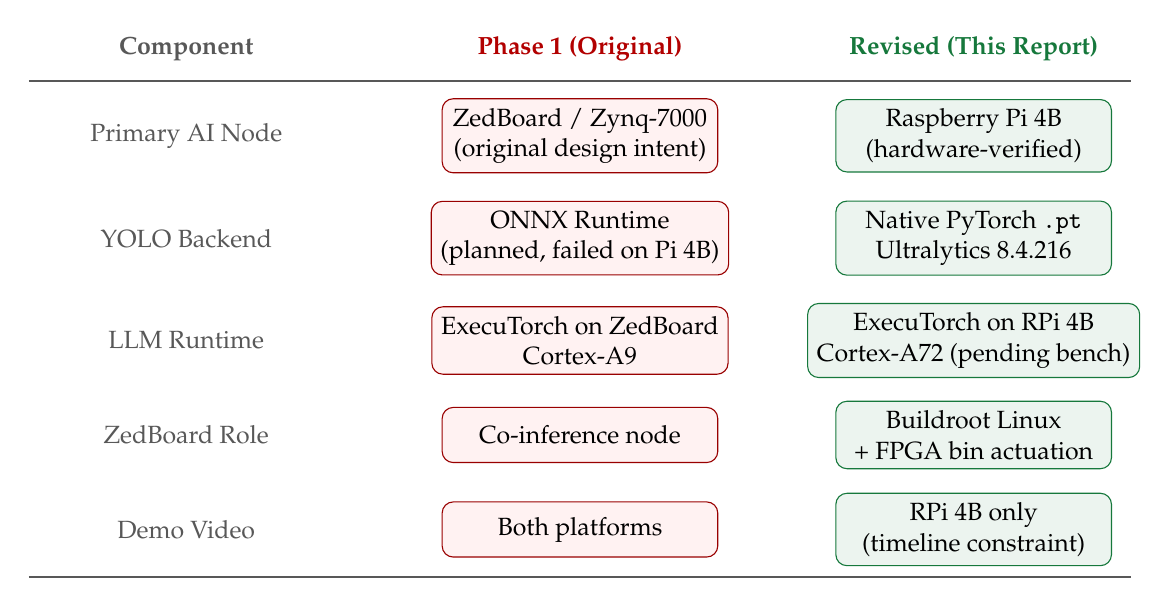
\begin{tikzpicture}[
  every node/.style={font=\small},
  box/.style={rectangle,rounded corners=4pt,draw,fill=white,
              minimum height=0.7cm,minimum width=3.5cm,align=center},
  redbox/.style={box,draw=red!60!black,fill=red!5},
  greenbox/.style={box,draw=ecosortgreen,fill=ecosortgreen!8},
  arrow/.style={->,>=Stealth,thick}
]
%% ── COLUMN HEADERS ───────────────────────────────────────────
\node[font=\bfseries\small,color=ecosortgray] at (0,0) {Component};
\node[font=\bfseries\small,color=red!70!black]       at (5,0) {Phase 1 (Original)};
\node[font=\bfseries\small,color=ecosortgreen]        at (10,0) {Revised (This Report)};

\draw[thick,color=ecosortgray] (-2,-0.4) -- (12,-0.4);

%% ── ROW 1: Primary AI ────────────────────────────────────────
\node[align=right,color=ecosortgray] at (0,-1.1) {Primary AI Node};
\node[redbox]   at (5,-1.1)  {ZedBoard / Zynq-7000\\(original design intent)};
\node[greenbox] at (10,-1.1) {Raspberry Pi 4B\\(hardware-verified)};

%% ── ROW 2: Inference Backend ─────────────────────────────────
\node[align=right,color=ecosortgray] at (0,-2.4) {YOLO Backend};
\node[redbox]   at (5,-2.4)  {ONNX Runtime\\(planned, failed on Pi 4B)};
\node[greenbox] at (10,-2.4) {Native PyTorch \texttt{.pt}\\Ultralytics 8.4.216};

%% ── ROW 3: LLM Runtime ───────────────────────────────────────
\node[align=right,color=ecosortgray] at (0,-3.7) {LLM Runtime};
\node[redbox]   at (5,-3.7)  {ExecuTorch on ZedBoard\\Cortex-A9};
\node[greenbox] at (10,-3.7) {ExecuTorch on RPi 4B\\Cortex-A72 (pending bench)};

%% ── ROW 4: ZedBoard Role ─────────────────────────────────────
\node[align=right,color=ecosortgray] at (0,-4.9) {ZedBoard Role};
\node[redbox]   at (5,-4.9)  {Co-inference node};
\node[greenbox] at (10,-4.9) {Buildroot Linux\\+ FPGA bin actuation};

%% ── ROW 5: Demo Video ────────────────────────────────────────
\node[align=right,color=ecosortgray] at (0,-6.1) {Demo Video};
\node[redbox]   at (5,-6.1)  {Both platforms};
\node[greenbox] at (10,-6.1) {RPi 4B only\\(timeline constraint)};

\draw[thick,color=ecosortgray] (-2,-6.7) -- (12,-6.7);
\end{tikzpicture}
\caption{Architecture Comparison: Phase 1 Original Design vs.\ Revised Hardware-Validated Design.
         Red columns show original intentions; green columns show the corrected, ground-truth
         implementation status.}
\label{fig:arch_comparison}
\end{figure}

\clearpage

%% ============================================================
\section{Raspberry Pi 4 Model B --- Hardware and OS Configuration}

\begin{verifiedbox}[Raspberry Pi 4B Setup]
All items in this section have been physically confirmed on hardware.
\end{verifiedbox}

\subsection{Hardware Specification}

\renewcommand{\arraystretch}{1.30}
\begin{table}[H]
\centering
\caption{Verified Raspberry Pi 4 Model B Hardware Configuration}
\label{tab:rpi_hw}
\small
\begin{tabularx}{\linewidth}{@{} L{4.5cm} X @{}}
\toprule
\thead{Component} & \thead{Verified Configuration} \\
\midrule
\rowcolor{rowgray}
Board Model          & Raspberry Pi 4 Model B Revision 1.5 \\
System-on-Chip       & Broadcom BCM2711 \\
\rowcolor{rowgray}
Processor            & Quad-core ARM Cortex-A72 @ 1.5\,GHz \\
Instruction Set      & 64-bit ARMv8.0-A (\texttt{aarch64}) \\
\rowcolor{rowgray}
System RAM           & 4\,GB LPDDR4-3200 SDRAM \\
Operating System     & Raspberry Pi OS (Debian Trixie / Debian 13) \\
\rowcolor{rowgray}
Linux Kernel         & Linux 6.6.x (64-bit) \\
C/C++ Compiler       & GCC 14.2.0 \\
\rowcolor{rowgray}
Python               & Python 3.13.5 \\
Primary Storage      & 32\,GB Class 10 UHS-I microSD card \\
\rowcolor{rowgray}
Camera               & iBall Face2Face Webcam C20.0 (USB 2.0) \\
Camera Device Nodes  & \texttt{/dev/video0}, \texttt{/dev/video1} \\
\bottomrule
\end{tabularx}
\end{table}

\subsection{Repository Setup and Virtual Environment}

\begin{lstlisting}[language=bash, caption={Repository cloning and virtual environment on Raspberry Pi 4B}]
# Clone the project repository
git clone https://github.com/keer9999/BHARATH-AI-SOC.git
cd BHARATH-AI-SOC

# Create a virtual environment with access to system-installed ARM64 packages
# (--system-site-packages is required because PyTorch is installed as a Debian package)
python3 -m venv --system-site-packages .venv
source .venv/bin/activate
\end{lstlisting}

\clearpage

%% ============================================================
\section{Python, OpenCV, PyTorch and Ultralytics Installation}

\begin{verifiedbox}[Python Stack on Raspberry Pi 4B]
All packages listed here are installed and import-verified on the physical device.
\end{verifiedbox}

\subsection{Installation Procedure}

Standard PyPI wheel installation encountered missing ARM64 wheels for Python 3.13.
Two alternative sources were used:

\begin{lstlisting}[language=bash, caption={PyTorch and Ultralytics installation on Raspberry Pi 4B}]
# Step 1: Debian-packaged PyTorch and TorchVision (ARM64 binary, pre-tested on Cortex-A72)
sudo apt update && sudo apt install -y \
    python3-torch python3-torchvision python3-numpy python3-opencv

# Step 2: Ultralytics YOLO framework from PiWheels ARM64 mirror
python -m pip install --no-deps \
    --index-url https://www.piwheels.org/simple ultralytics
\end{lstlisting}

\subsection{Verified Software Versions}

\renewcommand{\arraystretch}{1.30}
\begin{table}[H]
\centering
\caption{Verified Python Stack Versions on Raspberry Pi 4B}
\label{tab:pystack}
\small
\begin{tabularx}{\linewidth}{@{} L{3.5cm} L{3.0cm} X @{}}
\toprule
\thead{Package} & \thead{Version} & \thead{Source / Verification} \\
\midrule
\rowcolor{rowgray}
Python       & 3.13.5          & System Python 3 \\
PyTorch      & 2.6.0+debian    & Debian Trixie ARM64 official repo \\
\rowcolor{rowgray}
TorchVision  & 0.21.0          & Debian Trixie ARM64 official repo \\
NumPy        & 2.2.4           & Debian ARM64; tensor bridge verified \\
\rowcolor{rowgray}
Ultralytics  & 8.4.216         & PiWheels ARM64 wheel \\
OpenCV       & 4.10.x          & \texttt{python3-opencv} headless (Debian) \\
\bottomrule
\end{tabularx}
\end{table}

\subsection{Verification Smoke Test}

\begin{lstlisting}[language=python, caption={CPU tensor and import verification on Cortex-A72}]
import torch, numpy as np, cv2
from ultralytics import YOLO

# Tensor arithmetic (confirms ARMv8.0-A NEON SIMD is functional)
x = torch.tensor([[1.0, 2.0], [3.0, 4.0]])
a = np.zeros((2, 2), dtype=np.float32)
b = torch.from_numpy(a)
assert (x + b).shape == (2, 2)

print(f"PyTorch:    {torch.__version__}")
print(f"NumPy:      {np.__version__}")
print(f"OpenCV:     {cv2.__version__}")
print("SUCCESS: All imports and tensor arithmetic verified on Cortex-A72.")
\end{lstlisting}

\clearpage

%% ============================================================
\section{Webcam Integration and Verification}

\begin{verifiedbox}[USB Webcam on Raspberry Pi 4B]
Camera device enumeration and frame capture physically confirmed.
\end{verifiedbox}

\subsection{V4L2 Hardware Verification}

\begin{enumerate}[label=\textbf{\arabic*.}]
  \item Install Linux Video4Linux2 (V4L2) utilities:
  \begin{lstlisting}[language=bash]
sudo apt install -y v4l-utils fswebcam
  \end{lstlisting}

  \item Enumerate connected camera devices:
  \begin{lstlisting}[language=bash]
v4l2-ctl --list-devices
# Result: iBall Face2Face Webcam C20.0: /dev/video0, /dev/video1
  \end{lstlisting}

  \item Inspect supported pixel formats and resolutions:
  \begin{lstlisting}[language=bash]
v4l2-ctl -d /dev/video0 --list-formats-ext
# Confirmed: YUYV 4:2:2 at 640x480 @ 30.000 fps
  \end{lstlisting}

  \item Capture a physical test frame:
  \begin{lstlisting}[language=bash]
fswebcam -d /dev/video0 -r 640x480 --no-banner ~/webcam-test.jpg
# Result: Frame captured — exposure, focus, and colour confirmed.
  \end{lstlisting}
\end{enumerate}

\subsection{OpenCV Camera Integration}

\begin{lstlisting}[language=python, caption={OpenCV V4L2 camera integration (src/webcam\_capture.py)}]
import cv2

cap = cv2.VideoCapture(0, cv2.CAP_V4L2)
cap.set(cv2.CAP_PROP_FRAME_WIDTH, 640)
cap.set(cv2.CAP_PROP_FRAME_HEIGHT, 480)
cap.set(cv2.CAP_PROP_FPS, 30)

ret, frame = cap.read()
if ret:
    print(f"Frame shape: {frame.shape}")  # (480, 640, 3) confirmed
cap.release()
\end{lstlisting}

\clearpage

%% ============================================================
\section{YOLO Trained Weights and Model Selection}

\subsection{Trained Model Inventory}

The repository contains eleven trained YOLO weight files under \texttt{src/yolo/weights/}.

\renewcommand{\arraystretch}{1.30}
\begin{table}[H]
\centering
\caption{Trained YOLO Model Inventory}
\label{tab:models}
\small
\begin{tabularx}{\linewidth}{@{} L{5.2cm} C{1.6cm} C{2.2cm} X @{}}
\toprule
\thead{Model File} & \thead{Size} & \thead{Status} & \thead{Scope} \\
\midrule
\rowcolor{rowgray}
\texttt{ecosort\_waste\_yolo11s.pt}  & $\sim$21.5\,MB & \verified & \textbf{Primary: 66 classes, 7 categories} \\
\texttt{ecosort\_waste\_yolo11s.onnx}& $\sim$37\,MB   & \inprogress & ONNX export (opset 12; SIGILL on Pi 4B) \\
\rowcolor{rowgray}
\texttt{general\_waste.pt}           & $\sim$20.8\,MB & \configured & Mixed domestic waste \\
\texttt{plastic\_containers.pt}      & $\sim$21.0\,MB & \configured & Rigid plastics \\
\rowcolor{rowgray}
\texttt{bottle\_specialist.pt}       & $\sim$18.4\,MB & \configured & Bottles (clear, coloured, crushed) \\
\texttt{food\_organic.pt}            & $\sim$19.6\,MB & \configured & Biodegradable kitchen waste \\
\rowcolor{rowgray}
\texttt{plastic\_bag.pt}             & $\sim$18.9\,MB & \configured & Thin-film LDPE bags \\
\texttt{resin\_codes.pt}             & $\sim$22.1\,MB & \configured & RIC \#1--\#7 identification \\
\rowcolor{rowgray}
\texttt{ewaste\_a.pt}                & $\sim$20.4\,MB & \configured & PCBs, cables, components \\
\texttt{ewaste\_b.pt}                & $\sim$20.1\,MB & \configured & Batteries, smartphones, chargers \\
\rowcolor{rowgray}
\texttt{best.pt}                     & $\sim$21.5\,MB & \configured & Highest mAP@50 checkpoint \\
\bottomrule
\end{tabularx}
\end{table}

\subsection{Active Deployment Model}

The system is configured to load the primary unified model only:
\begin{lstlisting}[language=bash]
# Set the active model to the primary 66-class unified weights
export ECOSORT_CUSTOM_MODEL="$PWD/src/yolo/weights/ecosort_waste_yolo11s.pt"

# Single-model mode: bypass the 8 specialist models (~250 MB saved)
export ECOSORT_ONNX_ONLY=1
\end{lstlisting}

\clearpage

%% ============================================================
\section{ONNX Runtime Compatibility Issue and Native PyTorch Solution}

\begin{importantbox}
ONNX Runtime \textbf{cannot be deployed} on the Raspberry Pi 4 Model B.
Native PyTorch \texttt{.pt} execution via Ultralytics is the confirmed working approach.
\end{importantbox}

\subsection{The Original Plan}

ONNX Runtime was selected in the Phase 1 design as a lightweight inference backend
to reduce PyTorch framework overhead. YOLO11 models were exported to ONNX format
(opset 12, input shape $1 \times 3 \times 640 \times 640$) in preparation.

\subsection{The Failure: SIGILL on Import}

Upon installing the ARM64 ONNX Runtime package on Debian Trixie:

\begin{lstlisting}[language=bash, caption={ONNX Runtime fatal crash on Raspberry Pi 4B (Cortex-A72)}]
$ python -c "import onnxruntime"
Illegal instruction (core dumped)
\end{lstlisting}

\subsection{Root-Cause Analysis via GDB}

\begin{lstlisting}[language=bash, caption={GDB session identifying the illegal FP16 instruction}]
$ gdb --args python3 -c "import onnxruntime"
(gdb) run
Program received signal SIGILL, Illegal instruction.
0x0000ffff93a4b120 in ?? () from libonnxruntime.so
(gdb) x/i $pc
=> 0xffff93a4b120:    fmov    v25.4h, #0.5
\end{lstlisting}

\paragraph{Analysis.}
\texttt{fmov v25.4h, \#0.5} is an ARMv8.2-A half-precision (FP16) SIMD instruction.
The Cortex-A72 (BCM2711) implements \textbf{ARMv8.0-A} and does not support the
ARMv8.2-A FP16 vector extension. The prebuilt Debian ONNX Runtime binary was compiled
targeting a newer ARMv8.2-A baseline (e.g., Cortex-A76 in Raspberry Pi~5), making it
\textit{physically incompatible} with the Pi~4B. This is a binary distribution defect,
not a model or code defect.

\subsection{The Solution: Native PyTorch \texttt{.pt} Execution}

\begin{mdframed}[linecolor=ecosortgreen,linewidth=2pt,roundcorner=6pt,
                 backgroundcolor=ecosortgreen!5,skipabove=6pt,skipbelow=6pt,
                 innerleftmargin=10pt,innerrightmargin=10pt]
\textbf{Architectural Decision:} Use native PyTorch 2.6.0+debian with Ultralytics 8.4.216
to execute \texttt{.pt} weights directly. Both packages are compiled from Debian's ARM64
source tree targeting ARMv8.0-A and are fully operational on Cortex-A72 without any
illegal instruction traps.
\end{mdframed}

\begin{lstlisting}[language=python, caption={Native PyTorch YOLO11s inference on Raspberry Pi 4B}]
from ultralytics import YOLO

model = YOLO("src/yolo/weights/ecosort_waste_yolo11s.pt")
results = model.predict(source=0, conf=0.4, iou=0.5, device="cpu")
for r in results:
    for box in r.boxes:
        cls  = model.names[int(box.cls)]
        conf = float(box.conf)
        print(f"Detected: {cls} ({conf:.2%} confidence)")
\end{lstlisting}

\subsection{ONNX vs.\ PyTorch Comparison on Raspberry Pi 4B}

\renewcommand{\arraystretch}{1.30}
\begin{table}[H]
\centering
\caption{ONNX Runtime vs.\ Native PyTorch on Raspberry Pi 4B Cortex-A72}
\label{tab:onnx_vs_pt}
\small
\begin{tabularx}{\linewidth}{@{} L{4.0cm} X X @{}}
\toprule
\thead{Criterion} & \thead{ONNX Runtime} & \thead{Native PyTorch \texttt{.pt}} \\
\midrule
\rowcolor{rowgray}
Deployment Result  & \textbf{FAILED} (\texttt{SIGILL} on import) & \textbf{Operational} \\
Root Cause         & ARMv8.2-A FP16 binary incompatibility & ARMv8.0-A compatible binary \\
\rowcolor{rowgray}
Package Source     & Debian \texttt{python3-onnxruntime}     & Debian \texttt{python3-torch} \\
Memory Usage       & N/A (never ran)                         & $\sim$180\,MB single-model mode \\
\rowcolor{rowgray}
Expected Latency   & N/A                                     & 300--450\,ms/frame (expected) \\
Current Status     & \inprogress{}\ (source-build option)     & \verified \\
\bottomrule
\end{tabularx}
\end{table}

\clearpage

%% ============================================================
\section{YOLO, SAHI and NMS Detection Pipeline}

\subsection{Inference Pipeline Architecture}

The detection pipeline on the Raspberry Pi 4B follows a three-stage flow:

\begin{figure}[H]
\centering
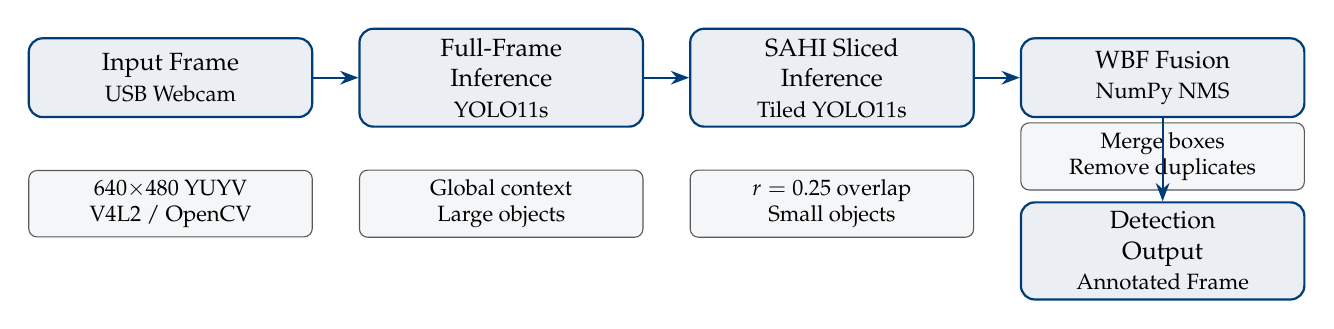
\begin{tikzpicture}[
  every node/.style={font=\small},
  node distance=0.0cm,
  stage/.style={rectangle,rounded corners=5pt,draw=ecosortblue,thick,
                fill=ecosortblue!8,minimum height=1.0cm,
                minimum width=3.6cm,align=center},
  detail/.style={rectangle,rounded corners=3pt,draw=ecosortgray,
                 fill=rowgray,minimum height=0.75cm,
                 minimum width=3.6cm,align=center,font=\footnotesize},
  arrow/.style={->,>=Stealth,thick,color=ecosortblue}
]

%% Row 1: Stage boxes (evenly spaced)
\node[stage] (input)  at (0,0)    {Input Frame\\{\footnotesize USB Webcam}};
\node[stage] (full)   at (4.2,0)  {Full-Frame\\Inference\\{\footnotesize YOLO11s}};
\node[stage] (sahi)   at (8.4,0)  {SAHI Sliced\\Inference\\{\footnotesize Tiled YOLO11s}};
\node[stage] (fusion) at (12.6,0) {WBF Fusion\\{\footnotesize NumPy NMS}};
\node[stage] (output) at (12.6,-2.2) {Detection\\Output\\{\footnotesize Annotated Frame}};

%% Row 2: detail boxes (below each stage)
\node[detail] at (0,-1.6)
  {640$\times$480 YUYV\\V4L2 / OpenCV};
\node[detail] at (4.2,-1.6)
  {Global context\\Large objects};
\node[detail] at (8.4,-1.6)
  {$r=0.25$ overlap\\Small objects};
\node[detail] at (12.6,-1.0)
  {Merge boxes\\Remove duplicates};

%% Arrows (horizontal)
\draw[arrow] (input.east)  -- (full.west);
\draw[arrow] (full.east)   -- (sahi.west);
\draw[arrow] (sahi.east)   -- (fusion.west);
\draw[arrow] (fusion.south) -- (output.north);

\end{tikzpicture}
\caption{EcoSort AI detection pipeline on Raspberry Pi 4B: webcam input $\rightarrow$
         full-frame YOLO11s $\rightarrow$ SAHI sliced YOLO11s $\rightarrow$ Weighted Box
         Fusion $\rightarrow$ annotated output.}
\label{fig:detect_pipeline}
\end{figure}

\subsection{SAHI Slicing Aided Hyper Inference}

Standard YOLO models miss small waste items (bottle caps, blister packs, pull-tabs)
in wide-angle bin views. The SAHI engine (\texttt{src/sahi\_detector.py}) addresses this:

\begin{enumerate}[label=\textbf{\arabic*.}]
  \item \textbf{Adaptive Slicing:} Frame divided into overlapping tiles of size
  $P\!\times\!Q$ with overlap ratio $r=0.25$;
  \item \textbf{Dual-Scale Inference:} YOLO11s runs on the full frame (global context)
  and each tile independently (fine resolution);
  \item \textbf{Coordinate Remapping:} Tile-local detections mapped back to global frame;
  \item \textbf{Weighted Box Fusion (WBF):} Custom pure-NumPy WBF merges overlapping
  detections across global and tile predictions without external library dependencies.
\end{enumerate}

\subsection{Expected Performance on Raspberry Pi 4B}

\renewcommand{\arraystretch}{1.25}
\begin{table}[H]
\centering
\caption{Expected Inference Performance on Raspberry Pi 4B (Pending Live Benchmark)}
\label{tab:perf}
\small
\begin{tabularx}{\linewidth}{@{} L{5.0cm} X X @{}}
\toprule
\thead{Metric} & \thead{YOLO11s Baseline} & \thead{YOLO11s + SAHI} \\
\midrule
\rowcolor{rowgray}
Latency / Frame  & 300--450\,ms (CPU, expected)    & 600--900\,ms (tiled) \\
Effective FPS    & 2.2--3.3\,FPS                   & 1.1--1.6\,FPS \\
\rowcolor{rowgray}
Small-Object Recall & Baseline                    & Target: $+$15\%--$+$25\% \\
RAM Working Set  & $\sim$180\,MB                   & $\sim$260\,MB \\
\rowcolor{rowgray}
Verification Status & \configured                 & \configured \\
\bottomrule
\end{tabularx}
\end{table}

\clearpage

%% ============================================================
\section{Llama 3.2 1B and ExecuTorch Development}

\begin{pendingbox}[ExecuTorch On-Device Execution]
The ExecuTorch engine module is \textbf{fully implemented}. On-device execution
and benchmarking on the Raspberry Pi 4B Cortex-A72 is the \textbf{immediate next
verification milestone}.
\end{pendingbox}

\subsection{Competition Mandate}

\begin{reqbox}[Mandatory PS-2 Requirement]
\textit{``A model from the Llama family must be used for the advisory or reasoning
component and deployed on-device using ExecuTorch as the reference runtime.''}
\end{reqbox}

\subsection{Model Selection: Llama 3.2 1B Instruct}

Llama~3.2~1B~Instruct is chosen for the following reasons:
\begin{itemize}
  \item At INT8 precision, it occupies $\sim$1.4\,GB RAM, leaving headroom for the
  vision pipeline on the Pi~4B's 4\,GB;
  \item Explicitly supported by ExecuTorch's ARM XNNPACK backend targeting Cortex-A series;
  \item Strong instruction-following for structured disposal advice and RIC code explanation.
\end{itemize}

\subsection{ExecuTorch Integration Status}

\renewcommand{\arraystretch}{1.30}
\begin{table}[H]
\centering
\caption{ExecuTorch Llama Integration Status}
\label{tab:executorch_status}
\small
\begin{tabularx}{\linewidth}{@{} L{5.5cm} C{2.5cm} X @{}}
\toprule
\thead{Work Item} & \thead{Status} & \thead{Notes} \\
\midrule
\rowcolor{rowgray}
Engine module (\texttt{executorch\_llama\_engine.py}) & \verified   & Implemented and import-verified \\
LLM wrapper interface (\texttt{llama\_engine.py})     & \verified   & Multi-backend: ExecuTorch + GGUF fallback \\
\rowcolor{rowgray}
Llama 3.2 1B \texttt{.pte} bundle export             & \configured & ARM XNNPACK delegate; pending download \\
On-device \texttt{.pte} execution on RPi 4B           & \inprogress & Next verification milestone \\
\rowcolor{rowgray}
Latency benchmark on Cortex-A72                       & \planned    & Target: 5--10 tokens/sec \\
GGUF fallback (\texttt{llama-3.2-1b-instruct-q4})     & \configured & Operational alternative \\
\bottomrule
\end{tabularx}
\end{table}

\subsection{ExecuTorch Engine Implementation}

\begin{lstlisting}[language=python, caption={ExecuTorch Llama Engine — implemented in src/executorch\_llama\_engine.py}]
class ExecuTorchLlamaEngine:
    """
    On-device Llama 3.2 1B via ExecuTorch ARM XNNPACK runtime.
    Satisfies mandatory reference runtime requirement for Bharat AI-SoC PS-2.
    Status: Module implemented; .pte on-device execution pending verification.
    """
    def __init__(self, pte_path="models/llama3_2_1B_xnnpack.pte"):
        self.pte_path = pte_path
        self._load_runtime()     # loads ExecuTorch runtime with XNNPACK delegate

    def generate_advice(self, item_name: str, category: str) -> str:
        prompt = (
            f"<|begin_of_text|><|start_header_id|>system<|end_header_id|>\n"
            f"You are EcoSort AI, an expert waste disposal assistant.\n"
            f"<|eot_id|><|start_header_id|>user<|end_header_id|>\n"
            f"Item: {item_name} (Category: {category}). Disposal advice?\n"
            f"<|eot_id|><|start_header_id|>assistant<|end_header_id|>\n"
        )
        return self._execute_pte(prompt)
\end{lstlisting}

\subsection{Deterministic Fallback: WasteAdvisor}

To guarantee $<$5\,ms disposal advice during ExecuTorch loading or under CPU load,
\texttt{src/waste\_advisor.py} provides a 2\,300-rule deterministic engine:
\begin{itemize}
  \item All Resin Identification Codes (\textbf{RIC \#1 through \#7});
  \item Contamination routing (food-soiled cardboard $\to$ composting);
  \item Hazardous material protocols (lithium batteries $\to$ e-waste isolation).
\end{itemize}

\clearpage

%% ============================================================
\section{Flask Dashboard, SQLite and Waste Advisory}

\begin{verifiedbox}[Application Software]
Flask application, SQLite schema, and WasteAdvisor are configured and import-verified.
Live end-to-end integration benchmarking is the next milestone.
\end{verifiedbox}

\subsection{Web Dashboard (\texttt{src/web\_app.py})}

\begin{lstlisting}[language=bash]
# Launch the web dashboard on Raspberry Pi 4B
source .venv/bin/activate
export ECOSORT_CUSTOM_MODEL="$PWD/src/yolo/weights/ecosort_waste_yolo11s.pt"
export ECOSORT_ONNX_ONLY=1
python src/web_app.py --port 5001
# Access at: http://<raspberry-pi-ip>:5001
\end{lstlisting}

\subsection{REST API Endpoints}

\renewcommand{\arraystretch}{1.30}
\begin{table}[H]
\centering
\caption{Flask REST API Endpoint Reference (port 5001)}
\label{tab:api}
\small
\begin{tabularx}{\linewidth}{@{} L{3.0cm} L{1.4cm} L{2.0cm} X @{}}
\toprule
\thead{Endpoint} & \thead{Method} & \thead{Response} & \thead{Description} \\
\midrule
\rowcolor{rowgray}
\texttt{/}             & GET  & HTML   & Dashboard: live stream, chat, analytics. \\
\texttt{/video\_feed}  & GET  & MJPEG  & Webcam with YOLO bounding-box overlays. \\
\rowcolor{rowgray}
\texttt{/api/status}   & GET  & JSON   & Camera, sensor, model, LLM health. \\
\texttt{/api/detect}   & POST & JSON   & Detection on uploaded image. \\
\rowcolor{rowgray}
\texttt{/api/chat}     & POST & JSON   & Disposal query; Llama / WasteAdvisor reply. \\
\texttt{/api/detections}& GET & JSON   & Detection history with class filter. \\
\rowcolor{rowgray}
\texttt{/api/stats}    & GET  & JSON   & Waste composition statistics. \\
\texttt{/api/sensors}  & GET  & JSON   & Pico~W sensor telemetry. \\
\bottomrule
\end{tabularx}
\end{table}

\clearpage

%% ============================================================
\section{ZedBoard Hardware Specifications}

\renewcommand{\arraystretch}{1.30}
\begin{table}[H]
\centering
\caption{Digilent ZedBoard Zynq-7000 XC7Z020 Hardware Specifications}
\label{tab:zedboard}
\small
\begin{tabularx}{\linewidth}{@{} L{4.5cm} X @{}}
\toprule
\thead{Component} & \thead{Specification} \\
\midrule
\rowcolor{rowgray}
SoC                    & Xilinx Zynq-7000 XC7Z020-CLG484-1 \\
Processing System (PS) & Dual-core ARM Cortex-A9 MPCore @ 667\,MHz \\
\rowcolor{rowgray}
PS Cache               & 32\,KB L1 I/D (per core); 512\,KB shared L2 \\
Programmable Logic (PL)& Artix-7 (85\,K logic cells; 53\,200 LUTs; 220 DSPs) \\
\rowcolor{rowgray}
System RAM             & 512\,MB DDR3 (32-bit bus @ 533\,MHz) \\
Non-Volatile Storage   & 256\,Mb Quad-SPI Flash + microSD slot \\
\rowcolor{rowgray}
Serial Interface       & USB-UART bridge (Cypress CY7C64225) \\
Network Interface      & Gigabit Ethernet PHY (Marvell 88E1518) \\
\rowcolor{rowgray}
User Peripherals       & 8 LEDs (LD0--LD7), 8 slide switches, 5 pushbuttons \\
Expansion              & 5$\times$ PMOD, FMC LPC, XADC header \\
\rowcolor{rowgray}
PS--PL Interface       & AXI Interconnect; AXI GPIO base address \texttt{0x41200000} \\
\bottomrule
\end{tabularx}
\end{table}

\clearpage

%% ============================================================
\section{Buildroot: Installation, Image Preparation and SD-Card Deployment}

\begin{verifiedbox}[Buildroot Embedded Linux]
Buildroot cross-compilation completed. Bootable microSD card written and partitioned.
Full hardware boot confirmation is in progress.
\end{verifiedbox}

\subsection{Why Buildroot?}

Buildroot was chosen over desktop distributions (Ubuntu Core, Linaro) for:
\begin{itemize}
  \item \textbf{Minimal footprint:} Root filesystem $<$20\,MB on 512\,MB DDR3;
  \item \textbf{Deterministic boot:} Kernel-to-userspace in $<$3.5\,seconds;
  \item \textbf{Full toolchain control:} GNU cross-compiler targeting Cortex-A9 + VFPv3;
  \item \textbf{Hardware co-design foundation:} Straightforward custom kernel driver and
  \texttt{devmem2} AXI GPIO register integration.
\end{itemize}

\subsection{Build and Deployment Workflow}

\begin{figure}[H]
\centering
\begin{tikzpicture}[
  every node/.style={font=\small},
  step/.style={rectangle,rounded corners=5pt,draw=ecosortblue,thick,
               fill=ecosortblue!8,minimum height=1.0cm,
               minimum width=2.9cm,align=center},
  arrow/.style={->,>=Stealth,thick,color=ecosortblue},
  status/.style={font=\footnotesize,color=statusgreen}
]
%% Six steps in two rows of three, properly spaced
\node[step] (s1) at (0,0)      {1. Configure\\{\footnotesize\texttt{zynq\_zed\_defconfig}}};
\node[step] (s2) at (3.8,0)    {2. Cross-Compile\\{\footnotesize Cortex-A9 Toolchain}};
\node[step] (s3) at (7.6,0)    {3. Generate Images\\{\footnotesize Kernel + U-Boot + rootfs}};
\node[step] (s4) at (7.6,-2.0) {4. Flash microSD\\{\footnotesize FAT32 BOOT + ext4}};
\node[step] (s5) at (3.8,-2.0) {5. UART Console\\{\footnotesize Minicom 115200\,8N1}};
\node[step] (s6) at (0,-2.0)   {6. Hardware Boot\\{\footnotesize U-Boot + Kernel}};

%% Status labels
\node[status] at (0,0.75)    {\checkmark~Done};
\node[status] at (3.8,0.75)  {\checkmark~Done};
\node[status] at (7.6,0.75)  {\checkmark~Done};
\node[status] at (7.6,-2.75) {\checkmark~Done};
\node[status] at (3.8,-2.75) {\checkmark~Done};
\node[color=statusamber,font=\footnotesize] at (0,-2.75) {$\circ$~In Progress};

%% Arrows
\draw[arrow] (s1.east)  -- (s2.west);
\draw[arrow] (s2.east)  -- (s3.west);
\draw[arrow] (s3.south) -- (s4.north);
\draw[arrow] (s4.west)  -- (s5.east);
\draw[arrow] (s5.west)  -- (s6.east);
\end{tikzpicture}
\caption{Buildroot Embedded Linux workflow for Digilent ZedBoard Zynq-7000.
Steps 1--5 are complete. Step 6 (hardware boot confirmation) is in progress.}
\label{fig:buildroot}
\end{figure}

\subsection{Build Commands}

\begin{lstlisting}[language=bash, caption={Buildroot cross-compilation commands (executed on host Ubuntu workstation)}]
# Install Buildroot dependencies
sudo apt install -y build-essential libncurses-dev wget git bc unzip

# Clone Buildroot source
git clone --depth=1 https://github.com/buildroot/buildroot.git
cd buildroot

# Load ZedBoard default configuration
make zynq_zed_defconfig

# (Optional) Customise kernel, BusyBox, and package selection
make menuconfig

# Cross-compile: kernel + U-Boot + BusyBox rootfs (takes 30-60 min)
make -j$(nproc)

# Output images are in buildroot/output/images/
# - uImage          : Linux kernel
# - u-boot.img      : U-Boot bootloader
# - rootfs.ext4     : Root filesystem
# - zynq-zed.dtb    : Device tree blob

# Flash to microSD (replace /dev/sdX with actual device)
sudo dd if=output/images/sdcard.img of=/dev/sdX bs=4M status=progress conv=fsync
\end{lstlisting}

\clearpage

%% ============================================================
\section{UART and Minicom Debugging}

\begin{verifiedbox}[UART Console]
Minicom serial console configured and connected to ZedBoard USB-UART bridge.
\end{verifiedbox}

\subsection{Setup}

\begin{lstlisting}[language=bash, caption={UART terminal setup for ZedBoard boot monitoring}]
# Install serial communication utilities on host workstation
sudo apt install -y minicom lrzsz

# Connect to ZedBoard USB-UART bridge (Cypress CY7C64225)
# Baud rate: 115200, Data: 8N1, No hardware flow control
minicom -D /dev/ttyACM0 -b 115200
# Alternative device node: /dev/ttyUSB0
\end{lstlisting}

\subsection{Expected Boot Sequence via UART}

The expected UART console output during a successful ZedBoard boot:
\begin{lstlisting}[language=bash, caption={Expected ZedBoard boot sequence (UART output)}]
# Stage 1: FSBL (First Stage Boot Loader)
Xilinx First Stage Boot Loader
Release 2024.1

# Stage 2: U-Boot
U-Boot 2024.01 (Zynq ZedBoard)
DRAM: 512 MiB
Loading kernel from SD ...

# Stage 3: Linux Kernel (Buildroot)
Booting Linux on physical CPU 0x0
Linux version 6.x (Buildroot cross-compiler)

# Stage 4: BusyBox Init
Starting kernel ...
Welcome to Buildroot
zedboard login:
\end{lstlisting}

\subsection{Current Boot Status}

\begin{pendingbox}[ZedBoard Hardware Boot]
The Buildroot image has been flashed and the UART console is connected. Early-stage
U-Boot handoff is under active debugging. A successful BusyBox login prompt will be
documented here upon confirmation.
\end{pendingbox}

\clearpage

%% ============================================================
\section{Planned: Ethernet Communication and FPGA Integration}

\begin{reqbox}[Development Roadmap]
Sections below describe planned work that follows ZedBoard boot confirmation.
\end{reqbox}

\subsection{Ethernet Communication: Raspberry Pi 4B $\leftrightarrow$ ZedBoard}

\begin{enumerate}[label=\textbf{E\arabic*.}]
  \item Configure DHCP or static IP on the ZedBoard Marvell 88E1518 GbE PHY;
  \item Verify TCP/IP socket connectivity with the Raspberry Pi 4B on the LAN;
  \item Implement a lightweight JSON-over-TCP classification packet protocol:
  the Pi~4B sends the detected waste category, the ZedBoard translates it to a
  bin index (1--7) and writes the AXI GPIO register.
\end{enumerate}

\subsection{FPGA AXI GPIO Bin Actuation}

\begin{enumerate}[label=\textbf{F\arabic*.}]
  \item Deploy the AXI GPIO peripheral driver (\texttt{hardware/zynq7000/axi\_gpio\_driver.py})
  using \texttt{devmem2} at base address \texttt{0x41200000};
  \item Map waste categories to LED outputs:
  \texttt{LD1}=Plastic, \texttt{LD2}=Glass, \texttt{LD3}=Metal,
  \texttt{LD4}=Paper, \texttt{LD5}=Organic, \texttt{LD6}=E-Waste, \texttt{LD7}=Hazardous;
  \item Confirm $<$1\,$\mu$s actuation latency via AXI interconnect register write.
\end{enumerate}

\clearpage

%% ============================================================
\section{Testing Results, Limitations and Future Work}

\subsection{Automated Test Results}

\renewcommand{\arraystretch}{1.30}
\begin{table}[H]
\centering
\caption{Automated Test Suite Results}
\label{tab:tests}
\small
\begin{tabularx}{\linewidth}{@{} L{4.0cm} C{2.0cm} C{2.5cm} X @{}}
\toprule
\thead{Test Suite} & \thead{Tests} & \thead{Result} & \thead{Scope} \\
\midrule
\rowcolor{rowgray}
Core unit tests (\texttt{tests/})
  & 58 & \textcolor{statusgreen}{\textbf{58/58 Pass}}
  & WasteAdvisor rules, SAHI, database, webcam, API. \\
Hailo backend simulation (\texttt{hardware/hailo\_npu/})
  & 13 & \textcolor{statusgreen}{\textbf{13/13 Pass}}
  & HailoRT inference class (CPU-simulated). \\
\rowcolor{rowgray}
Live webcam inference
  & ---  & \inprogress{}
  & End-to-end latency and FPS pending. \\
ExecuTorch on-device benchmark
  & ---  & \inprogress{}
  & Tokens/sec on Cortex-A72 pending. \\
\bottomrule
\end{tabularx}
\end{table}

\subsection{Known Limitations}

\begin{enumerate}[label=\textbf{L\arabic*.}]
  \item \textbf{ONNX Runtime:} Cannot be deployed via prebuilt Debian ARM64 binary on
  Cortex-A72. A source-build targeting ARMv8.0-A is a potential future option.
  \item \textbf{ExecuTorch Benchmarking:} The \texttt{.pte} bundle requires the
  \texttt{llama3\_2\_1B\_xnnpack.pte} model file to be downloaded and placed in \texttt{models/}.
  On-device execution timing has not yet been recorded.
  \item \textbf{ZedBoard Boot:} Full Linux boot confirmation is pending UART debug resolution.
  \item \textbf{Inference FPS:} The Cortex-A72 without a hardware accelerator is expected to
  deliver 2--3\,FPS for live detection; real-time 30\,FPS requires a Hailo-8 NPU.
  \item \textbf{Demo Video Scope:} The submission video demonstrates the Raspberry Pi 4B
  node only, due to timeline constraints on ZedBoard bring-up.
\end{enumerate}

\subsection{Future Work}

\begin{enumerate}[label=\textbf{W\arabic*.}]
  \item Confirm ZedBoard boot and deploy AXI GPIO bin actuation driver;
  \item Complete ExecuTorch on-device benchmark on Raspberry Pi 4B;
  \item Record live inference FPS and latency metrics;
  \item Establish RPi 4B $\leftrightarrow$ ZedBoard Ethernet communication;
  \item Optionally: source-compile ONNX Runtime for ARMv8.0-A to validate ONNX export;
  \item Add Hailo-8 AI HAT\texttt{+} for $>$30\,FPS real-time vision if hardware is available.
\end{enumerate}

\clearpage

%% ── References ───────────────────────────────────────────────
\begin{thebibliography}{99}

\bibitem{arm2026bharatai}
Arm Developer Labs,
``Bharat AI-SoC Challenge 2026--27: PS-2,'' 2026.
\url{https://arm-education.github.io/Arm-Developer-Labs/Bharat_AI_SoC_2026_27.html}

\bibitem{ultralytics2024yolo11}
G.~Jocher and J.~Qiu, ``Ultralytics YOLO11,'' v8.3.0, 2024.
\url{https://github.com/ultralytics/ultralytics}

\bibitem{meta2024llama3}
Meta AI, ``Llama 3.2: Edge-Optimised Open Foundation Models,'' 2024.
\url{https://ai.meta.com/blog/llama-3-2-connect-2024/}

\bibitem{pytorch2024executorch}
PyTorch Team, ``ExecuTorch: On-Device AI Runtime,'' Linux Foundation, 2024.
\url{https://pytorch.org/executorch}

\bibitem{xnnpack2024}
Google LLC, ``XNNPACK: Neural Network Inference for ARM,'' 2024.
\url{https://github.com/google/XNNPACK}

\bibitem{akyon2022sahi}
F.~C.~Akyon, S.~O.~Altinuc, A.~Temizel,
``Slicing Aided Hyper Inference for Small Object Detection,''
\emph{IEEE ICIP 2022}, pp.~966--970.

\bibitem{xilinx2023zynq}
AMD Xilinx, ``Zynq-7000 SoC Technical Reference Manual (UG585),'' 2023.

\bibitem{raspberrypi2024pi4b}
Raspberry Pi Ltd, ``Raspberry Pi 4 Model B Documentation,'' 2024.
\url{https://www.raspberrypi.com/documentation/computers/raspberry-pi.html}

\bibitem{buildroot2024}
The Buildroot Project, ``Buildroot: Making Embedded Linux Easy,'' 2024.
\url{https://buildroot.org}

\end{thebibliography}

\end{document}
